%This is an example for a chapter, additional chapter can be added in the skeleton-thesis
%To generate the final document run latex, build and quick build commands on the skeleton-thesis file not this one.
\chapter{Introduction}

%As many have discovered, they are not 100\% accurate and many applications are used for a significant amount of time prior to being removed from the market.  With this immense number of applications, comes many requests for access to varying types of data on the phone some of which is may not be required to function.


Within the smartphone market, there are three primary flavors, iOS, Android, and Blackberry.  At present, Android is the most popular smartphone operating system comprising approximately 75\% of the global smartphone market~\cite{Perez} and bosting an application ecosystem that recently passed 700,000 applications~\cite{Womack}.  Unfortunately, popularity has not been isolated to users alone.  No more than 10 years ago smartphone malware did not exist.  Today, there have been 69,000~\cite{networkworld} reported instances of malware on the Google Play market alone.  While their are commercially available anti-virus applications, none of them are widely used and their methods are not understood due to their closed nature.  At present, user's primarily depend on Google and other Android markets to adequately identify malware.  Unlike the Apple iOS ecosystem whose applications are centrally verified before becoming available, Android applications are more lightly vetted.  This puts more responsibility on the user to make the important decision of which applications they trust.  The permissions architecture employed by Android, however, makes these trust decisions more difficult.  

%\subsection{Android Background}
%Because the quality and trustworthiness of applications varies widely, Android treats all applications as potentially buggy or malicious.  Every application runs as an unprivileged user with Linux UIDs effectively being used to provide application sandboxes only permitting applications to access their own files by default.  To increase code re-usability, the Android application framework forces a component-based application model~\cite{4768655}.  Instead of having a main() function or any single entry point for execution, Android applications are developed in terms of components.  The applications are composed of four component types:  activity, service, broadcast receiver, and content provider.  Activities are focused windows in which the user interaction takes place; only one activity can be active at a time.  Each activity is a class in the source code and should perform according to events generated by the user and system.  Services are designed to run in the background while content providers manage access to data.  Broadcast Receivers are registered with system services and can receive system events, such as re-boot completed, or an SMS received, etc.  Once a broadcast receiver is registered to receive a system event, the code specified in the broadcast receiver is run whenever the system event is triggered.  Most system events are guarded by permissions, which the applications must declare and get approval for at installation time.  All permissions are requested by the application developer in a manifest which is incorporated into the application package, and approved by the user when the application is installed.  

  

\subsection{Mobile Device Permission Models}

In the current implementation, application developers are responsible for defining the set of permissions their application “requires” independent of what their application’s code actually uses~\cite{Felt}.  The list is presented to the user at install-time whether installing an application obtained through the Google Play market or elsewhere.  This list contains the canonical names given to each permission object, but provides little context as to what the permission is being utilized for.  At the end of the day, users have no choice but to accept all of the permissions or not install the application; they can't grant or deny specific permissions.

While all smartphone applications are susceptible to being over permissioned, Apple's iOS and Blackberry's OS both give the user the ability to revoke an application’s permissions.  iOS uses a "dynamic" permissions model; the user is prompted once per application to use phone features such as the GPS receiver.  The user then has the option of changing their decision through the system's settings menu.  

Blackberry OS uses a "static" approach similar to that of Android.  Application developers declare the set of permissions they would like their program to have, and this list is presented to the user at installation.  However, unlike Android, the user has the option to edit the list and revoke any permission.  This approach adds a degree of granularity to an otherwise binary trust decision and gives the user more control over which applications they trust to access their data.  This study will explore implementing this approach in the Android OS.  

\subsection{Removing Permissions from Android Apps}

Shown in Figure~\ref{fig:permission}, is the application permissions listing for a Flashlight application obtained through the Play market.  While one would reason that this application should only need the hardware controls necessary to turn on the phone's light, due to the large quantities of ad network libraries and other debris embedded within, it asks for much more.  If permissions were editable, the user would be able to trust this application’s ability to operate the flashlight without having to worry about the true reason for the other permission requests.  
\FloatBarrier
\begin{figure}[h!]
\centerline{\resizebox{0.3\linewidth}{!}{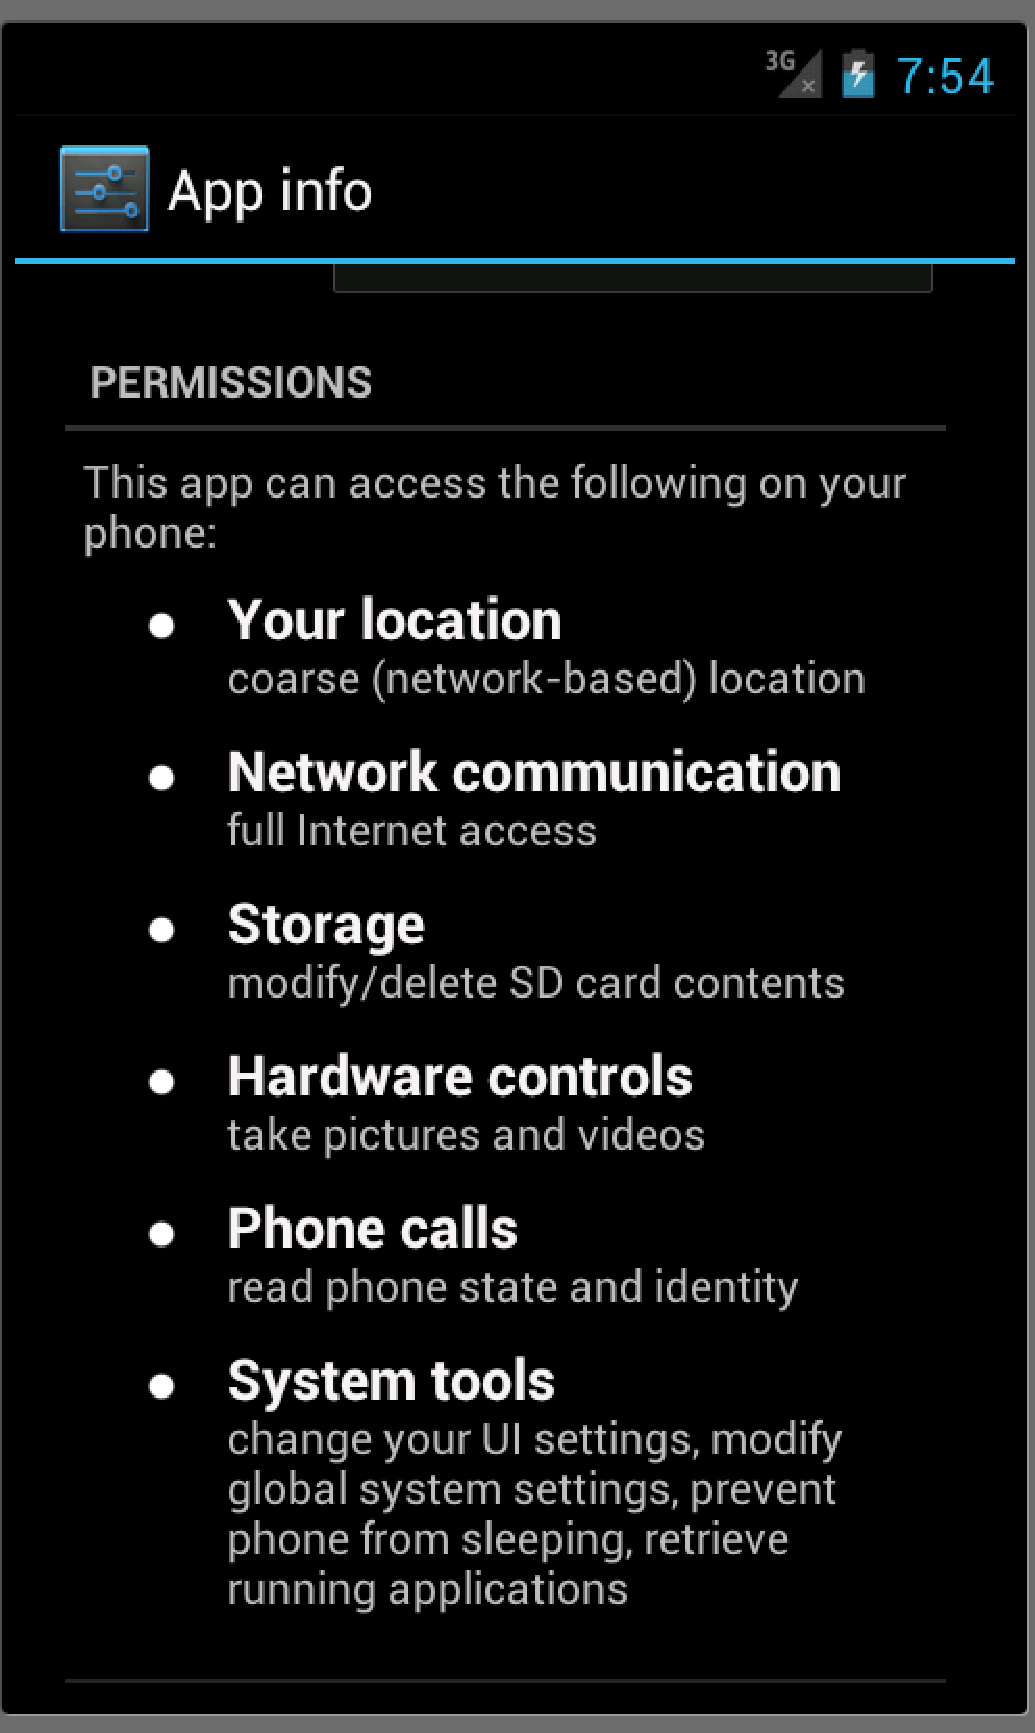
\includegraphics{figure1}}}
\caption{Flashlight app permission requirements}
\label{fig:permission}
\end{figure}
\FloatBarrier
There are various ways one could remove permissions from Android applications.  Previous work in this area proposes a "privacy mode", where applications running in this mode run with lowered permissions~\cite{Zhou:2011:TISSA}.  This approach requires heavy modification to the Android OS itself, but yields a flexible solution.  Applications can also be repackaged, with their manifests modified to contain fewer permissions.  This is the most popular approach at present, as applications containing this functionality can be readily obtained from major application markets~\cite{Hoffman}.  Additionally, the application's executable code could be dynamically rewritten to protect sensitive API calls~\cite{Davis:2013:RetroSkeleton}.  

All of the above approaches, however, are dependent on Google's policy regarding application permissions, as they influence how developers write their applications.  Google's documentation discusses the implementation in enough detail for a developer to use it, but does not go into the rationale behind the approach.  While they do suggest that the "dynamic" permission model would be too much of a burden on the user, they do not mention editable static permissions at all.  Furthermore, application developers are not explicitly instructed to handle cases of revoked permissions in their applications.  Since the lack of a required permission is typically implemented in the form of a Java SecurityException~\cite{Google}, some programmers will handle these gracefully out of habit.  However, if an application or library it uses is not explicitly written to handle the permission revocation, modification of the source code will be required to ensure proper function.  

\subsection{Effect of Permission Removal}

While previous research has demonstrated that a significant number of Android applications request and use too many permissions~\cite{Felt}, it is unclear how removing permissions would affect the application's behavior.  Under Android's security model, developers typically expect all the requested permissions to be available.  Therefore, it would not be surprising if many developers do not handle the lack of permissions gracefully.  When an application invokes an API call without the necessary permissions, it typically throws a \texttt{SecurityException}.  However, if such an exception is caught by library or wrapper code, the application can continue running.  Moreover, permissions are not all equal.  Some permissions describe a devices' hardware capabilities, such as \texttt{CAMERA}.  Since they are not universally available, one would expect libraries to be able to handle their absence more gracefully.  A relatively common instance of this is the removal of the camera on DoD phones for operational security.  

When removing a permission, users will expect to see any correlating features disabled, a common scenario being the removal of GPS capabilities from Google Maps.  Currently, many users turn their GPS off in attempts to extend their battery life.  When this is done, at launch, the user is notified that the accuracy of Google Maps would be improved if GPS was enabled.  When removing permissions from an application, users are going to expect similar behavior.  If an application was not written with permission removal in mind, however, features that are not obviously correlated may malfunction leaving the user confused.  Theoretically, if the application is not written to handle its data in a robust manner, this could include data corruption.  If this is the case, data would be susceptible to being corrupted if the application crashes regardless of permission removal.  While these occurrences are of concern, in the long run, they can easily be addressed by developers.  

This study takes the first step towards quantitatively measuring the effects of removing permissions from Android applications.  While removing a permission may cause many abnormal behaviors, this study focuses on crashes, which is likely the most common.  Seven permissions that have a high potential of compromising a user's security or privacy will be tested in attempts to answer the following questions:

\begin{itemize}
\item What is the likelihood an application crash after a permission is removed?

\item Which permissions, if removed, are less likely to cause an application to crash?

\item Why do applications handle the lack of certain permissions more gracefully?

\end{itemize}

This work will benefit both users and developers.  Users can make more informed decisions when deciding which permissions to remove (when they use tools for removing permissions).  Application developers can make their code more robust against missing permissions.  Android library developers can design their libraries to handle the potential lack of permissions more gracefully.  
	
%The remainder of this paper will attempt to quantify the effects of removing permissions from Android applications.  In Chapter \ref{sec:related}, related work will be discussed.  Then, in Chapter \ref{sec:methodology}, the methodology and the tool that was developed for automated testing, PyAndrazzi, will be discussed.  The results of the testing are presented in Chapter \ref{sec:evaluation} and the impact of the findings on users and developers is discussed in Chapter \ref{sec:discussion}.  Finally, in Chapter \ref{sec:future} future work is discussed and Chapter \ref{sec:conclusion} concludes.  
